\documentclass[12pt]{article}

\usepackage{amsmath}
\usepackage{gensymb}
\usepackage{standalone}
\usepackage{verbatim}
\usepackage[utf8]{inputenc}
\usepackage{setspace}
\usepackage[a4paper,margin=1in,footskip=0.25in]{geometry}
\usepackage{graphicx}
\usepackage{mathptmx}
\usepackage{booktabs}
\usepackage{cite}
\usepackage[english]{babel}
\usepackage[utf8]{inputenc}
\usepackage{setspace}
\usepackage{url}
\usepackage{titlepic}

\title{Finite Element Approximation of Poisson's Equation for Determination of Internal Voltages}
\titlepic{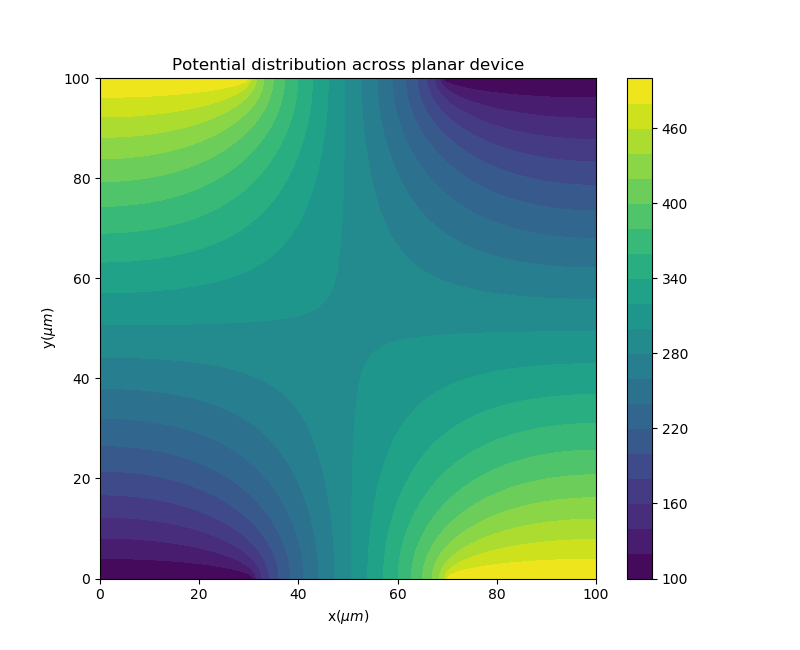
\includegraphics[width=\linewidth]{4_terminal.png}}
\author{Alan Burl}
\date{\today}

\begin{document}

	\maketitle
	\clearpage
	%\documentclass[12pt]{article}
%
%\usepackage{amsmath}
%\usepackage{gensymb}
%\usepackage{standalone}
%\usepackage{verbatim}
%\usepackage[utf8]{inputenc}
%\usepackage{setspace}
%\usepackage[a4paper,margin=1in,footskip=0.25in]{geometry}
%\usepackage{graphicx}
%\usepackage{mathptmx}
%\usepackage{booktabs}
%\usepackage{cite}
%\usepackage[english]{babel}
%\usepackage[utf8]{inputenc}

\begin{document}
\section{Problem Statement}
	The determination of the potential field in a detector leads by way of weighting potential to the determination of theoretical pulse output. The determination of this is done by solving Poisson's equation. This proves to be difficult, if not impossible, for geometries other than simple cases. To solve these geometries, a finite element approach can be taken and implemented to solve nearly any geometry. This work details the implementation of the finite approach to solve Poisson's equation to solve a three terminal device.
\end{document}
%	\input(Theory.tex}
	\documentclass{article}[12pt]
\usepackage{amsmath}
\usepackage{gensymb}
\usepackage{standalone}
\usepackage{verbatim}
\usepackage[utf8]{inputenc}
\usepackage{setspace}
\usepackage[a4paper,margin=1in,footskip=0.25in]{geometry}
\usepackage{graphicx}
\usepackage{mathptmx}
\usepackage{booktabs}
\usepackage{cite}
\usepackage[english]{babel}
\usepackage[utf8]{inputenc}

\begin{document}
\section{Development of Matrices and solution}
	Using input from the user interface, a matrix of dimension $nxm$ with $n$ and $m$ being the number specified in the $x$ and $y$ directions. The spaing and placement of the nodes is done using Python3.7 NumPy module. Nodes of the geometry are broken down into boundary conditions and field conditions. 
\subsection{Boundary Conditions}
	Boundary condition locations are taken form the user interface by means of the terminal geometry widget. In this widget, the geometric location and size of the terminal is entered as well as the potential applied across the terminal. At this point, the terminal is limited to having an uniform distribution across the entire surface. These inputs are passed as arguments to the boundary condition method of Voltage Calculation class in Calculation.py. The specified voltage is used as the boundary condition and is placed assigned to its respective location in the $b$ matrix. The remainder of the boundary conditions are determined by use of ?????. This mirrors the adjacent node on the same axis for finite approximation. For a terminal with known potential on the right side of the geometry, an example is shown in (\ref{eq:right_boundary}).
	
	\begin{equation}
		\frac{\partial{^2V}}{\partial{x^2}}+\frac{\partial{^2V}}{\partial{y^2}} \approx \frac{\left(V_{x+1}-V_{xy}\right)-\left(V_x-V_{x+1}\right)}{\Delta x^2}+\frac{\left(V_{y-1}-V_{xy}\right)-\left(V_{xy}-V_{y+1}\right)}{\Delta y^2}=V_{ap}
		\label{eq:right_boundary}
	\end{equation}
	
Where $V_{xy}$ is the boundary node being evaluated, and $\Delta x$, $\Delta y$ are the distance between nodes in the $x$ and $y$ directions respectively. (\ref{eq:right_boundary}) is reduced to have a coefficient of one for the node in question for matrix solving, seen in (\ref{eq:reduced_boundary}).
	\begin{equation}
		V_{xy}-\frac{V_{x+1}\Delta y^2}{\Delta x^2+\Delta y^2}-\frac{V_{y-1}\Delta x^2}{\Delta  x^2+\Delta y^2}-\frac{V_{y+1}\Delta x^2}{\Delta  x^2+\Delta y^2}=\frac{-\rho \Delta  x^2 \Delta y^2}{2\epsilon\left(\Delta x^2+\Delta y^2\right)}
		\label{eq:reduced_boundary}
	\end{equation}
The remainder of the boundary conditions are solved using the same method with their respective nodes. 
\subsection{Field Conditions}
	After determination of the boundary conditions is complete, the field of the geometry is calculated. All nodes in the field are determined using (\ref{eq:field_values}).  The implementation of a space charge term, $\rho$, can be done in this process. 
	\begin{equation}
		V_{xy}-\frac{V_{x+1}\Delta y^2}{2\left(\Delta x^2+\Delta y^2\right)}-\frac{V_{x-1}\Delta y^2}{2\left(\Delta x^2+\Delta y^2\right)}-\frac{V_{y-1}\Delta x^2}{2\left(\Delta  x^2+\Delta y^2\right)}-\frac{V_{y+1}\Delta x^2}{2\left(\Delta  x^2+\Delta y^2\right)}=\frac{-\rho \Delta  x^2 \Delta y^2}{2\epsilon\left(\Delta x^2+\Delta y^2\right)}
		\label{eq:field_values}
	\end{equation}
\subsection{Calculation}
	After all nodes in the matrix have been accounted for, the A matrix will have ones on the diagonal with other constituents on the same row. Use of Python3.7 NumPy module is used to solve for the voltage vector. This vector is returned to the user interface by means of a contour plot.
\end{document}

	\documentclass{article}[12pt]
\usepackage{amsmath}
\usepackage{gensymb}
\usepackage{standalone}
\usepackage{verbatim}
\usepackage[utf8]{inputenc}
\usepackage{setspace}
\usepackage[a4paper,margin=1in,footskip=0.25in]{geometry}
\usepackage{graphicx}
\usepackage{mathptmx}
\usepackage{booktabs}
\usepackage{cite}
\usepackage[english]{babel}
\usepackage[utf8]{inputenc}

\begin{document}
\section{Code Validation}
	To verify the functionality and accuracy of the implemented code a simple two terminal device was used. The geometry was set to be a $100\mu m$ square with $100$ nodes on each axis. The terminals were placed across the top and bottom surfaces, with the top having an applied voltage of $1000V$ and the bottom being set to ground. Solving of Poisson's equation for this geometry results in a linear relationship. \\ \\
 	\noindent
 The simulated results of the two terminal device is seen in Figure \ref{fig:two_terminal}. As can be seen the simulated results show a linear relationship between voltage and distance in $y$.
 
 \begin{figure}[h!]
 	\centering
 	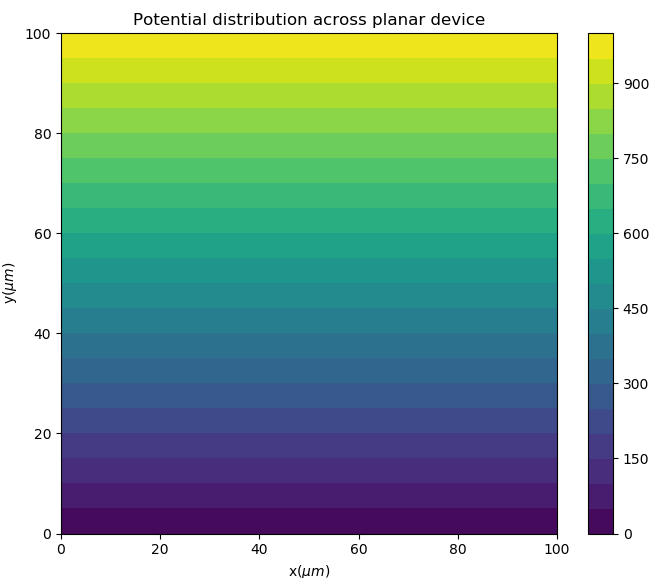
\includegraphics[width=\linewidth]{two_terminal1.png}
 	\caption{Simulated voltage distribution of two terminal device.}
 	\label{fig:two_terminal}
\end{figure}
\end{document}

	\documentclass{article}[12pt]
\usepackage{amsmath}
\usepackage{gensymb}
\usepackage{standalone}
\usepackage{verbatim}
\usepackage[utf8]{inputenc}
\usepackage{setspace}
\usepackage[a4paper,margin=1in,footskip=0.25in]{geometry}
\usepackage{graphicx}
\usepackage{mathptmx}
\usepackage{booktabs}
\usepackage{cite}
\usepackage[english]{babel}
\usepackage[utf8]{inputenc}

\begin{document}
\section{Results}
Having verified the functionality of the code, a three terminal device was simulated. The device was $100\mu m$ square with $100$ nodes an each axis. The first terminal was placed on the bottom of the plate and spanned $100\mu m$ at a potential of 30V.  The second terminal was located a $y=100\mu m$ and spanned $30\mu m$ in the postive x-direction at a potential of 100V. The last terminal was located at $y=100\mu m$ and $x=70\mu m$ and spanned $30 \mu m$ at a potential of 0V. The resulting contour plot is seen in Figure \ref{fig:three_terminal}.
\begin{figure}[h!]
	\centering
	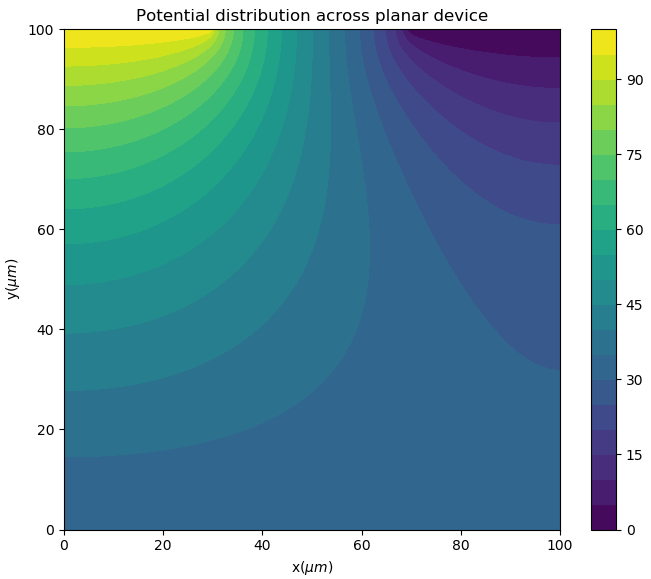
\includegraphics[width=\linewidth]{three_terminal.png}
	\caption{Simulated applied voltage of three terminal device detector geometry.}
	\label{fig:three_terminal}
\end{figure}
\end{document}

	\section{Code Usage}
		The code used in the development of this can be found on GitHub at \url{https://github.com/alangburl/Finite_Element_Votlage.git}. It is also included in the included zip file. The code was developed using Python3.7.1 and PyQt5. Functionality of this code is not guaranteed if deployed using older/newer software. The package needed for calculation, NumPy, is included with many popular scientific distributions of Python, including Anaconda. Launching and execution of the code should be done via command line. Execution of this code in Spyder will result in erratic behavior.
	%\clearpage
	%\bibliographystyle{unsrt}
	%\bibliography{bibliography}


\end{document}